\subsection{MOSFET}\label{ssec:mosfet}
	First of all, MOSFET stands for Metal-Oxide-Semiconductor-Field-Effect-Transistor. The main characterisc of the MOSFET that makes it stand from other field effect transistors is that the MOSFET gate is electrically insulated from the main current carrying channel as Figure \ref{fig:mosfet-structure} shows. 

		\begin{figure}[htbp]
			\centering
			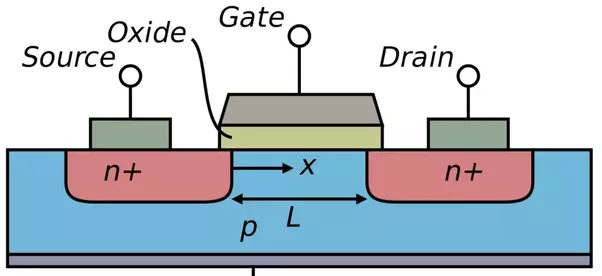
\includegraphics[scale=0.5]{figuras/fig-mosfet-structure.png}
			\caption{MOSFET structure \cite{mosfet-structure}}
			\label{fig:mosfet-structure}
		\end{figure}

	MOSFETs are three terminal devices with a Gate, a Drain and a Source. The two main types of MOSFETs are N-channel (PMOS) and P-channel (NMOS), each having different features. In NMOS transistors, the silicon channel between the source and drain is of p-type silicon. When a positive voltage is placed on the gate electrode, it repulses the holes in the p-type material forming a conducting (pseudo n-type) channel and turning the transistor on. A negative voltage turns the transistor off. With a PMOS transistor, the opposite occurs. A positive voltage on the gate turns the transistor off, and a negative voltage turns it on. NMOS transistors switch faster than PMOS \cite{et-mosfet}. 
	\par
	According to \cite{radio-mosfet} there are basically three regions in which MOSFETs can operate:

	\begin{itemize}
		\item\textit{\textbf{Cut-off region:}} In this region of the MOSFET is in a non-conducting state, channel current ($I_{DS}$) = 0. The gate voltage (V$_{GS}$) is less than the threshold voltage ($V_{T}$) required for conduction.\label{itm:mosfet-cutoff-region}
		\item\textit{\textbf{Linear region:}} In this linear region the channel is conducting and controlled by the gate voltage. For the MOSFET to be in this state the (V$_{GS}$) must be greater than the threshold voltage ($V_{T}$) and also the voltage across the channel ($V_{DS}$), must be greater than V$_{GS}$ minus $V_{T}$.\label{itm:mosfet-linear-regior}
		\item\textit{\textbf{Saturation region:}} In this region the MOSFET is turned hard on. The voltage drop for a MOSFET is typically lower than that of a bipolar transistor and as a result power MOSFETs are widely used for switching large currents.\label{itm:mosfet-saturation-region}
	\end{itemize}
